\section{Análisis Bivariado}

\newcommand{\varnorm}[1] {
    (#1_t - \mu_{\lowercase{#1}})
}

\newcommand{\squarederr}[1]{
    \sum\limits_{t=1}^n \varnorm{#1}^2
}

\newcommand{\crosscorr}[2]{
  \frac{\sum\limits_{t=|k|+1}^n \varnorm{#1} (#2_{t-|k|} - \mu_{#2})}{
    \sqrt{\squarederr{#1} \squarederr{#2}}
  } \\
}

Para medir cuánto se ``mimetizan'' las dos series, utilizaremos la función de correlación cruzada (c.c.f), que mide cuánto se parecen la serie $X$ e $Y$ aplicando un desplazamiento $k$, dándonos un valor entre $-1$ y $1$ (similar a la correlación de la estadística clásica).

Podemos aproximar la c.c.f. mediante la fórmula de la correlación cruzada muestral.

\begin{equation}
  r_{AB}(k) =
  \left\{
    \begin{array}{ll}
      \crosscorr{A}{B} & \mbox{si } k \geq 0 \\
      \crosscorr{B}{A} & \mbox{si } k < 0
    \end{array}
  \right.
\end{equation}

Podemos ver que, si $k \geq 0$, lo que hacemos es, a grandes rasgos, calcular la correlación de Pearson entre $A_{t+k}$ e $B_t$. Si $k < 0$, lo hacemos entre $A_t$ e $B_{t+k}$.

Para cada tarea, calculamos un correlograma cruzado para $k \in \{-6, -5, \ldots, 0, \ldots , 6\}$. Los valores de $k \geq 0$ los podemos considerar como aquellos en los cuales nos estamos fijando si $B$ se mimetiza con $A$, y aquellos $k \leq 0$ al revés. Luego, definimos

\begin{align}
  A \rightarrow B &= max \{ r_{AB}(k), k \leq 0 \} \\
  B \rightarrow A &= max \{ r_{AB}(k), k \geq 0 \} \\
\end{align}


$A \rightarrow B$ es el entrainment direccional de $A$ hacia $B$, que mide cuánto se mimetiza $B$ a $A$. (explicar un poco más ésto)

\begin{figure}
\centering
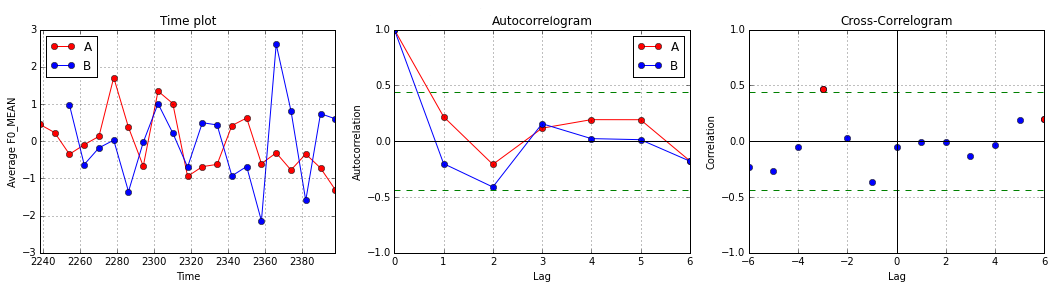
\includegraphics[width=15cm]{images/time_plot_with_cross_correlation.png}
\caption{Time-plot producido por TAMA, junto a su autocorrelación y correlación cruzada\label{time_plot_with_bivariate}}

\end{figure}
